\subsection{Utledning av bølgeligningen}
\subsubsection{Forhåndsbetingelser}
For å finne frem til bølgeligningen må en se på hvordan systemet en skal bruke likningen i ser ut.
På en gitar er lengden på strengen justerbar, men en endrer tonen ved å stramme eller slakke
på gitarstrengen.

En gitarstreng kan modelleres som en tråd som er spent mellom to punkter, der den er fiksert på plass.
I normaltilstand ligger strengen spent i en rett linje mellom punktene, frem til den blir plukket. Da
har den blitt forstyrret, og strengen begynner å vibrere. Problemet er da å finne en \(u(x,t)\) som modellerer
defleksjonen til strengen. Hvis strengen har lengde \(l\), massetetthet \(\rho\) og blir sluppet løs ved \(t=0\),
vil formelen finne defleksjonen til strengen for hvilken som helst \(x\) når \(t>0\).

Forutsetninger for løsning av bølgelikningen:

\begin{enumerate}
  \item Gravitasjon er neglisjerbar i forhold til strengspenningen.
  \item Alle defleksjoner er små og skjer i samme plan.
  \item Massen per lengde er konstant over hele strengen, slik at spenningen er den samme
  gjennom hele strengen.
\end{enumerate}

\subsubsection{Utledning}

\begin{figure}[H]
  \centering
  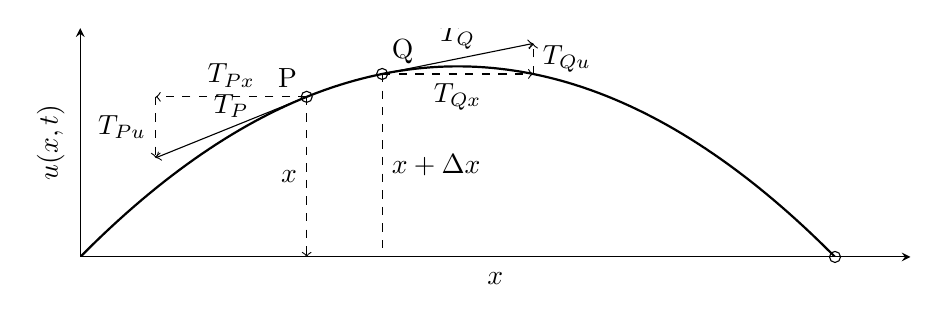
\begin{tikzpicture}
    \begin{axis}[
      width=\textwidth,
      height=0.37\textwidth,
      axis lines=left,
      xlabel={$x$},
      ylabel={$u(x,t)$},
      xmin=0, xmax=1.1,
      ymin=0, ymax=0.6,
      xtick=\empty,
      ytick=\empty
    ]

      % punkter
      \coordinate (Ppoint)  at (axis cs:0.3,0.42);
      \coordinate (Pupoint) at (axis cs:0.1,0.26);
      \coordinate (Pxpoint) at (axis cs:0.1,0.42);
      \coordinate (Qpoint)  at (axis cs:0.4,0.48);
      \coordinate (Qupoint) at (axis cs:0.6,0.56);
      \coordinate (Qxpoint) at (axis cs:0.6,0.48);

      % strengkurve
      \addplot[domain=0:1, samples=100, thick] {-2*x^2 + 2*x};

      % krefter ved P
      \draw[->, thin] (Ppoint) -- (Pupoint) node[midway, above] {$T_P$};
      \draw[->, thin, dashed] (Ppoint) -- (Pxpoint) node[midway, above] {$T_{Px}$};
      \draw[->, thin, dashed] (Pxpoint) -- (Pupoint) node[midway, left]  {$T_{Pu}$};

      % krefter ved Q
      \draw[->, thin] (Qpoint) -- (Qupoint) node[midway, above] {$T_Q$};
      \draw[->, thin, dashed] (Qpoint) -- (Qxpoint) node[midway, below] {$T_{Qx}$};
      \draw[->, thin, dashed] (Qxpoint) -- (Qupoint) node[midway, right] {$T_{Qu}$};

      % loddrette hjelpelinjer
      \draw[->, dashed] (axis cs:0.3,0.42) -- (axis cs:0.3,0) node[midway, left] {$x$};
      \draw[dashed]     (axis cs:0.4,0.48) -- (axis cs:0.4,0) node[midway, right] {$x+\Delta x$};

      % punktsymboler og etiketter
      \addplot[only marks, mark=o] coordinates {(0.3,0.42) (0.4,0.48) (1,0)};
      \node[anchor=south east] at (Ppoint) {P};
      \node[anchor=south west] at (Qpoint) {Q};
      \node[anchor=north]      at (axis cs:1,0) {$l$};

    \end{axis}
    \end{tikzpicture}
  \caption{Krefter og vinkler på et lite strengstykke \([x,\,x+\Delta x]\).}
\end{figure}

For å finne uikningen brukes en liten bit av strengen ved \(t=0\), som er \(\Delta x\) lang og starter på
\(x\). Punktet \(P=(x,u(x,0))\) og punktet \(Q=(x+\Delta x, u(x+\Delta x,0))\) er endene av strengstykket på strengen.
\(T\) er kraften som spenningen i strengen skaper på ett punkt \(x>0\) langs strengen. 
\(\alpha\) er vinkelen mellom \(T_{Qx}\) og \(T_Q\), og \(\beta\) er vinkelen mellom
\(T_{Px}\) og \(T_P\).

\begin{align*}
  T_{Px} = T_P \cos\beta, &\qquad T_{Qx} = T_Q \cos\alpha,\\
  T_{Pu} = T_P \sin\beta, &\qquad T_{Qu} = T_Q \sin\alpha.
\end{align*}

Fordi spenningen i strengen er lik over hele strengen, vil de horisontale kreftene
av \(T_Q\) og \(T_P\) utjevne hverandre:

\begin{equation}
  T_{Px} = T_{Qx} = T = \text{const.}
  \label{eq:horisontaleKrefterKonstant}
\end{equation}

Ifølge Newtons andre lov \((F=ma)\) sett på strengstykket, kan massen settes lik\(m=\rho\,\Delta x\) og
aksellerasjonen \(a=u_{tt}\). Kraften som blir påført strengen er \(F=T_{Qu}-T_{Pu}\). Da blir stykket slik:

\begin{equation*}
  T_{Qu}-T_{Pu}=\rho\,\Delta x\,\frac{\partial^2 u}{\partial t^2}.
\end{equation*}

Deretter kan \(\tan\theta=\frac{\sin\theta}{\cos\theta}\) og \eqref{eq:horisontaleKrefterKonstant} settes sammen, samtidig
antas \(\tan\alpha\) og \(\tan\beta\) til å være minimal, slik at en kan bruke forenklinger. De antas små fordi
i forutsetningene for bølgelikningen blir alle defleksjoner satt til å være små. 

\begin{equation}
  \frac{T_{Qu}}{T_{Qx}}-\frac{T_{Pu}}{T_{Px}}
  = \tan\alpha - \tan\beta
  = \frac{\partial u}{\partial x}(x+\Delta x,t)-\frac{\partial u}{\partial x}(x,t)
  = \frac{\rho\,\Delta x}{T}\,\frac{\partial^2 u}{\partial t^2}.
  \label{eq:krefterPaStykke}
\end{equation}

Gange begge sider med \(\dfrac{T}{\rho\,\Delta x}\):

\begin{equation}
  \frac{\partial^2 u}{\partial t^2}
  = \frac{T}{\rho\,\Delta x}\left[
     \frac{\partial u}{\partial x}(x+\Delta x,t)-\frac{\partial u}{\partial x}(x,t)
    \right].
  \label{eq:tidPartiellDerivert}
\end{equation}

Settes \(\Delta x\to 0\) som en grenseverdi, kommer definisjonen av den deriverte frem:

\begin{equation}
  \frac{\partial^2 u}{\partial t^2}
  = \lim_{\Delta x\to 0}\frac{T}{\rho}\frac{1}{\Delta x}
    \left[\frac{\partial u}{\partial x}(x+\Delta x,t)-\frac{\partial u}{\partial x}(x,t)\right]
  = \frac{T}{\rho}\,\frac{\partial^2 u}{\partial x^2}.
  \label{eq:deltaXGarMotNull}
\end{equation}

Settes \(c^2=\dfrac{T}{\rho}\) kommer bølgelikningen frem: 

\begin{equation}
  \frac{\partial^2 u}{\partial t^2}
  = c^2\,\frac{\partial^2 u}{\partial x^2},
  \qquad
  c^2=\frac{T}{\rho}.
  \label{eq:utledetBolgelikning}
\end{equation}

\subsection{Metode og verktøy for numerisk løsning}
\subsubsection{Valg av verktøy}
For å løse bølgelikningen numerisk, har vi valgt å bruke Python. Dette er et programmeringsspråk som er mye brukt innenfor vitenskapelige
beregninger, og har et stort utvalg av biblioteker som gjør det enkelt å implementere numeriske metoder og visualisere resultater. Innenfor 
bibliotekene numpy og matplotlib finnes det mange funksjoner som gjør det enkelt å løse oppgaver numerisk og plotte visuelle fremstillinger.
Dette gjør Python til et godt valg for å løse bølgelikningen numerisk. For å lage animasjoner av resultatene, har vi valgt å bruke biblioteket 
matplotlib.animation, som er en del av matplotlib-biblioteket. Dette lar brukeren få en bedre forståelse av hvordan løsningen utvikler seg over tid.
For å plotte grafen har vi brukt matplotlib.pyplot, som er et vanlig grafikkbibliotek i Python. Dette biblioteket gjør det enkelt å lage 2D-grafer og 
visualisere data. For å forstå komplekse lignigner som bølgeligningen er essensielt å kunne visualisere resultatene på en enkel måte.

\subsection{Løsning med separasjon av variable}
\begin{equation}
	u_{tt} = c^2 u_{xx} \qquad \iff \qquad 
	\frac{\partial^2 u}{\partial t^2} = \frac{T}{\rho} \frac{\partial^2 u}{\partial x^2}	
	\label{eq:bølgelikningForLøsning}
\end{equation}

En løsning av bølgeligningen forutsetter definerte rand- og initialbetingelser. Strengen har en fast lengde $l$,
og er festet i begge ender, dette er randbetingelsene. Initialbetingelsene skjer ved $t=0$, og da blir strengen
sluppet løs av en kraft, som har påvirket strengen til å slippes fra en posisjon bestemt av $f(x)$.
Ettersom strengen blir sluppet, er den partiellderiverte av $t$ ved $t=0$ $u_t(x,0) = 0$.

Grensebetingelsene for funksjonen $u(x,t)$ blir derfor:

\begin{align}
	u(0 , t) = 0 \label{eq:grensebetingelse0}\\
	u(l , t) = 0 \label{eq:grensebetingelsel}
\end{align}

og initialbetingelsene for funksjonen $u(x,t)$ blir:

\begin{align}
	u(x , o) &= f(x) = \sum_{n=0}^{n=\infty} c_n \sin \left( \frac{n \pi}{l} x \right) 	
	\label{eq:initialbetingelse1}
\end{align}

Separasjon av variabler går ut på å finne to funksjoner $F(x)$ og $G(t)$, der de tilsammen blir $u(x , t)$. 
Da får vi separert tid $t$ og posisjon $x$ i to ulike funksjoner.

\begin{equation*}
	u(x , t) = F(x)G(t)
\end{equation*}

De partiellderiverte av $F(x)$ og $G(t)$ vil derfor bli slik:

\begin{equation}
	u_{tt} = F(x)G''(t), \qquad u_{xx} = F''(x)G(x)
	\label{eq:separasjonPartiellDeriverte}	
\end{equation}

Fyller vi de partiellderiverte (\ref{eq:separasjonPartiellDeriverte}) inn i bølgelikningen (\ref{eq:bølgelikningForLøsning}):

\begin{align*}
  \hspace{35ex}
  u_{tt} &= c^2 u_{xx} \\
  \hspace{2ex} F(x)G''(t) &= c^2 F''(x)G(t) \hspace{10ex} \vert 
  \cdot \frac{1}{c^2 F''(x) G''(t)} \\
  \frac{F''(x)}{F(x)} &= \frac{1}{c^2} \frac{G''(t)}{G(t)}
\end{align*}

For at begge sider skal være like for alle verdier av $x \in \left[ 0 , l \right]$ og $t < 0$, må siste 
likningen være lik en konstant verdi. Denne verdien settes til $- \lambda^2$. Den må være negativ for 
at det skal bli et sinus og cosinus svar, og ikke et eksponentiellt svar. For å vise at konstanten alltid 
er positiv, er den opphøyd i andre.
Det kan skrives slik:

\begin{equation*}
	\frac{F''(x)}{F(x)} = \frac{1}{C^2} \frac{G''(t)}{G(t)} = - \lambda^2
\end{equation*}

$F(x)$ og $G(t)$ er blitt to ulike differensiallikninger som kan løses. Vi starter med $F(x)$ for der
kan grensebetingelsene (\ref{eq:grensebetingelse0}) og (\ref{eq:grensebetingelsel}) brukes for 
løsningen.

\begin{align*}
	\hspace{20ex} \frac{F''(x)}{F(x)} &= - \lambda^2 \hspace{10ex} \vert \cdot F(x)\\
	F''(x) + \lambda^2&F(x) = 0
\end{align*}

Løses dette som en 2. ordens homogen differensiallikning blir stykket slik:

\begin{align*}
	F''(x) + \lambda^2&F(x) = 0 \\ 
	\Rightarrow r^2 + &\lambda^2 = 0 \\
	\Rightarrow r_1 = 0 - i \lambda &\vee r_2 = 0 + i \lambda \\
	\Rightarrow F(x) = e^{0 \cdot x} & \left( \alpha  \cos \lambda x + \beta \sin \lambda x \right) \\
	\Rightarrow F(x) = \alpha \cos& \lambda x + \beta \sin \lambda x 
\end{align*}

Da kan grensebetingelse (\ref{eq:grensebetingelse0}) settes inn i likningen:

\begin{align*}
	u(0 , t) = F(&0)G(t) = 0\\
	\Rightarrow F(0) = \alpha \cos&\lambda \cdot 0 + \beta \sin \lambda \cdot 0 \\
	\Rightarrow F(0) = \alpha \cos&0 + \beta \sin 0 \\
	\Rightarrow F(0) = &\alpha = 0 \\
	\Rightarrow \alpha =& 0 \\
	\Rightarrow F(x) = &\beta \sin \lambda x
\end{align*}

Videre kan grensebetingelse (\ref{eq:grensebetingelsel}) settes inn for å finne verdien til $\lambda$.

\begin{align*}
	u(l ,t) = F(l&)G(t) = 0 \\
	\Rightarrow F(l) =& 0 \\
	\Rightarrow \beta \sin \lambda &\cdot l = 0 \\ 
	\Rightarrow \lambda = \frac{\pi n}{l}&, \qquad n \in \mathbb{N} \\
	\Rightarrow F(x) = { \beta }_n & \sin \frac{\pi n}{l} x
\end{align*}

Nå er uttrukket for $\lambda$ og $F(x)$ funnet, og neste seg er å finne uttrykket for $G(t)$:

\begin{align*}
	G''(t) = - \lambda^2 & c^2 G(t) \\
	\Rightarrow G''(t) + \lambda^2 & c^2 G(t) = 0 
\end{align*}

Deretter løses dette som en 2. ordens homogen differensiallikning.

\begin{align*}
	G''(t) + \lambda^2 & c^2 G(t) = 0 \\
	\Rightarrow r^2 + \lambda^2 c^2 = 0 \\
	\Rightarrow r_1 = 0 + i \lambda c &\vee r_2 = 0 - i \lambda c \\ 
	\Rightarrow G(t) = e^{0 t} \gamma&\cos c \lambda t + \psi \sin c \lambda t \\
	\Rightarrow G(t) = \gamma\cos & c \lambda t + \psi \sin c \lambda t
\end{align*}

Ettesom at strengen slippes fra startposisjonen som initialbetingelse (\ref{eq:initialbetingelse1})
bestemmer, er startfarten til strengen i høyderetning $u_t(x,0) = 0$. Ettersom det er $ \psi \sin c \lambda t $
som beskriver startfarten, blir dette satt lik $0$, og $G(t)$ blir slik:

\begin{equation*}
	G(t) = \gamma \cos c \lambda t = \gamma \cos \frac{c \pi n}{l} t
\end{equation*}

Settes uttrykkene for $F(x)$ og $G(t)$ sammen, blir løsningen til bølgelikningen slik:

\begin{equation}
	u(x,t) = \sum_{n=0}^{\infty} c_n 
	\sin \left( \frac{n \pi}{l} x \right)
	\cos \left( \frac{n \pi c}{l} t \right)
	\label{eq:bølgelikningLøst}	
\end{equation}

\subsubsection{Konstanten \texorpdfstring{$c_n$}{cn}}

Konstanten $c_n$ beskriver initialbetingelsene en løser bølgelikningen for. For en streng med lengde
$l$ av funksjonen $f(x)$ beskriver slik $u(x,0) = f(x)$, blir konstanten $c_n$ slik:

\begin{equation}
	c_n = \frac{2}{l} \int_{0}^{l} f(x) \sin \left( \frac{n \pi}{l} x \right) \,dx
	\label{eq:cnDefinisjon}
\end{equation}

\subsubsection{Beskrivelse av maple kode}

Maple koden starter med å definere initialbetingelsene for simuleringen Strengen er $l = 64,77cm$ lang, og blir dratt
opp i punkt $x = a = 7cm$ til høyde $u(a,0) = h = 2cm$. For å finne tettheten til gitarstrengene er 
formelen $\rho = 7825 kg/m^3 \cdot \pi (0.00256 \cdot string\_gauge /2)^2$. Strengtykkelsene er hentet fra tykkelsen til
Earnie Ball sine super slinky strengsett \parencite{ErnieBallSlinky}, og $7825 kg/m^3$ er massetetthet 
for stål ifølge wikipedia \parencite{WikipediaTetthet}, da det blir antatt at alle strengene 
er stålstrenger. Ved beregning av spenningskraft ble en streng-spennings-kalkulator-nettside 
\parencite{RodrigoStringTensionCalc} brukt, og ``0.009 D'Addario / Ernie Bal''  ble valgt som strenger på 
nettsiden. Deretter blir funksjonene for $f(x)$, $c_n$, og $u(x,t)$ definert, og en \verb|explore| og
\verb|plot| blir brukt for å plotte alle strengene på en graf, der en kan styre $t$ med en glider.
Ettersom det ikke var mulig å få inn navnet på de ulike strengene i plottet blir det vanskelig å 
skille de ulike strengene fra hverandre.

\subsection{Beskrivelse av kode for numerisk løsning}
\subsubsection{Pakker, variabler og parametere}
I dette delkapittelet skal vi se på en numerisk tilnærming til bølgeligningen, koden for simuleringen kan hentes fra 
følgende kilde: \parencite{simuleringKode}. 

Først importeres nødvendige pakker for å kunne utføre numeriske beregninger og plotte grafiske fremstillinger. Her
tar vi i bruk numpy for numeriske operasjoner, matplotlib.pyplot for plotting, og matplotlib.animation for å lage 
animasjoner slik som forklart i forrige seksjon. Deretter setter vi konfigurajsonsparametere som definerer
fysiske egenskaper til strengen, samt parametere for den numeriske løsningen. Dette inkluderer lengden $L$ på strengen,
bølgehastigheten $c$ og tiden $s$ vi ønsker å simulere. Videre defineres antall punkter $N$ som skal brukes til å dele 
opp strengen. Dette påvirker nøyaktigheten til den numeriske løsningen, der flere punkter gir en mer nøyaktig løsning,
men øker beregningstid og ressursbruk. Videre definerer vi modi for funksjonen, som er antall bølgetopper som skal være 
tilstede for å lage startformen, hvor en høyere verdi gir skarpere kanter og høyere detaljnivå. 

Videre setter vi opp betingelser for den grafiske fremstillingen, slik som FPS (frames per second) for animasjonen, og
tykkelsen for linjen på grafen. For å sette startformen på grafen setter vi 

\begin{lstlisting}
  initial_shape_type = "pluck"
  pluck_width: float = 0.15
\end{lstlisting}

hvor \verb|"pluck"| indikerer at grafen (i dette tilfellet en streng) skal strekkes, og \verb|pluck_width| definerer hvor bredt området som strekkes er.

\subsubsection{Initialbetingelser funksjonen}
Hensikten med denne funksjonen er å definere startformen til strengen ved $t=0$, som vil si at funksjonen returnerer $u(x,0)$.
Funksjonen tar inn en parameter \verb|x|, som er en numpy array med posisjoner langs strengen. Avhengig av verdien til
\verb|initial_shape_type|, vil funksjonen returnere forskjellige startformer. I dette tilfellet er det \verb|"pluck"| 
som er implementert som vil gi funksjonen en trekant-/teltformet startform, hvor plukkposisjonen bestemmes av følgende 
kode:

\begin{lstlisting}
  if initial_shape_type == "pluck":
    center = pluck_position * length_m
    width = pluck_width * length_m
    return np.clip(1.0 - np.abs(x - center) / width, 0.0, 1.0)
\end{lstlisting}

hvis du setter inn for verdi i vi har satt i starten av koden, vil dette si at strengen blir plukket slik som 
illustrert i figuren nedenfor:

\begin{figure}[H]
    \centering
    \begin{tikzpicture}
        \begin{axis}[
        width=0.9\textwidth,
        height=0.5\textwidth,
        axis lines=left,
        xlabel={$x$ [m]},
        ylabel={$u(x,0)$ [m]},
        xmin=0, xmax=1.02,
        ymin=-1.1, ymax=1.1,
        xtick={0.15, 0.45, 1},
        ytick={-1, 0, 1}
        ]
        
        \draw (0,0) -- (0.15,0);
        \draw [dashed] (0.15,0) -- (0.3,1) -- (0.45,0);
        \draw (0.45,0) -- (1,0);
        \fill (0.3,1) circle (2pt);

        \end{axis}
    \end{tikzpicture}
    \caption{Startform av strengen ved $t=0$ når den blir plukket ved $x=0.3$ m.}
\end{figure}

her ser vi at strenger blir plukket i en trekantformet bølge med høyde $y=1.0m$, og bredde på $0.15$ m. Dette er
ikke nøyaktig slik en streng ville sett ut hvis den ble plukket, men det gir en god tilnærming som er enkel å 
implementere i en numerisk modell.

Videre i koden setter vi startfarten til strengen ved $t=0$, som i dette tilfellet er null over hele strengen. Funksjonen som returneres vil 
derfor se slik ut: $g(x)=u_t(x,0)$ og vil returneres for alle verdier av $x$ som er gitt som input til funksjonen. Siden starthastigheten er satt
til $0$, vil \verb|return np.zeros_like(x)| returnere en array med samme form som \verb|x|, men med alle verdier satt til null.

\subsubsection{Oppsett av romlige og tidsmessige akser}
Først linje i denne kodebiten (\verb|np.ndarray x|)setter opp et array av jevnt fordelte punkter mellom $0$ og lengden $L$. Disse punktene vil da representere
posisjonene langs strengen hvor vi beregner $u(x,t)$. Eksempelvis hvis \verb|num_points=5| og \verb|length_m=1.0|, vil arrayet til \verb|x| se slik ut: \verb|x = [0, 0.25, 0.5, 0.75, 1.0]|.
Videre definerer vi \verb|float dt|, for å bergne avstand til naboer. Denne delen av koden er ikke i bruk, men lagt inn for fremtidsformål. Neste 
linje i koden (\verb|float dt|) definerer tidssteg til et bilde per sekund i animasjonen, hvor for \verb|fps=60| vil evaluere tilstanden hvert
$\frac{1}{60} \approx 16.7$ millisekund. Videre er beregning av antall tidssteg (\verb|num_steps = int(duration_s * fps) + 1|). Her vil varigheten
av simulasjonen og antall \verb|fps| bestemme hvor mange tidssteg som er i animasjonen slik at simuleringen var like lenge som animasjonen. Til
slutt har vi tiden \verb|np.ndarray t| som blir et array over alle tider hvor strengen skal beregnes.

\subsubsection{Metodefunksjonen}
I denne funksjonen settes simuleringen i gang. Grafen begynner å bevege seg som følge av de initialbetingelsene som ble definert tidligere. 
Bevegelsen oppstår gjennom stegvise beregninger av strengens utslag over tid. I denne funksjonen settes de ulike komponentene i ligningen
under:

\begin{equation*}
  u(x,t) = \sum_{n=1}^{N} 
  \big[ B_n \cos(\omega_n t) + B_n^{*} \sin(\omega_n t) \big]
  \sin\!\left(\frac{n\pi x}{L}\right)
\end{equation*}

Det første vi gjør er å hente startform \verb|f| og starthastighet \verb|g| ved å bruke initialbetingelser-funksjonene vi har definert tidligere. Videre lager vi en kolonnevektor med
modusindekser. Så bygger vi alle basisfunksjonene $\sin(\frac{n \pi x}{L})$ for alle $n$ og $x$ verdier. Resultatet av dette blir en matrise med $N (moduser) \cdot Nx (rompunkter)$. Videre
setter vi egenfrekvensener $\omega_n = c \frac{n \pi}{L}$ for en streng med faste ender.

Neste bit med kode regner ut fourier-koeffisientene fra f og g. Her tar vi i bruk formlene:

\begin{align*}
  B_n &= \frac{2}{L} \int_{0}^{L} f(x)\,\sin\!\left(\frac{n\pi x}{L}\right)\,dx \\
  B_n^{*} &= \frac{2}{L\,\omega_n} \int_{0}^{L} g(x)\,\sin\!\left(\frac{n\pi x}{L}\right)\,dx
\end{align*}

Neste kodebit allokerer en matrise for alle tidssteg, hvor tiden er i radene og rompunktene $x$ er i kolonnene. Deretter bergner vi de tidsavhengige koeffisientene for hvert tidspunkt $t_k$.
Her utrfører \verb|coeff_t @ sin_basis| summen $\sum_n a_n(t_k) \sin(\frac{n \pi x}{L})$ som gir $u(x, t_k)$ for alle $x$. Koden vil da bli seende slik ut:

\begin{lstlisting}
  frames = np.zeros((num_steps, num_points))
  for k, tk in enumerate(t):
      coeff_t = B * np.cos(omega_n * tk) + B_star * np.sin(omega_n * tk)
      frames[k, :] = coeff_t @ sin_basis
\end{lstlisting}

Etter dette tvinger vi randbetingelser $u(0, t) = u(L, t) = 0$ numerisk for å sikre robusthet, siden vi bruker \verb|np.trapz|-funksjonen som gir en tilnærmet verdi og \verb|num_modes=60| og
ikke går $\rightarrow \infty$. Så returnerer vi hele tidsutviklingen $u(x, t_k)$

\subsubsection{Animasjonsfunksjonen}
Her starter vi med å ta inn alle simulerte rammer, som er 2D-array med form \\ 
\verb|(num_steps, num_points)|, i tillegg til en tittel. Så oppretter vi figur og akse
før vi tegner første tidsramme som en linje og lagrer den i en variabel, som oppdateres for hver frame av animasjonen. Så setter vi x-aksen til strengens lengde, setter 
y-aksen ut i fra høyeste og laveste y-verdi for alle tider med litt ekstra padding lagt inn. Videre setter vi aksenavn, tittel, og tidsetikett som oppdateres underveis.
Så tegner vi selve startbildet med \verb|init()|-funksjonen, før vi oppdaterer funksjonen over tid med \verb|update(i)|-funksjonen. Til slutt bruker vi en innebygd funksjon
fra matplotlib.animation biblioteket som håndterer animasjonen videre, og ser slik ut:

\begin{lstlisting}
  anim = FuncAnimation(
    fig,
    update,
    frames=range(0, len(frames), 1),
    init_func=init,
    interval=1000 / (0.25* fps),
    blit=True,
    )
\end{lstlisting}

Her legger vi egentlig bare inn funksjonene sammen med noen paramtere for avspilling av animasjonen. Resten av koden er bare lagring av animasjonen lokalt og stillbilde 
for $t=0$.